\section{preliminaries}\label{sec:pre}
In this section, we first introduce some preliminaries on general hash tables and then present the background on the GPU architecture. 

\begin{table}
	\centering
	\caption{Frequently Used Notations}
	\vspace{-1.5em}
	\label{tbl:stat:datasets}
	\begin{tabular}{|c|l|}
		\hline
		$(k,v)$ & a key value pair \\ \hline
		$d$		& the number of hash functions \\ \hline
		$h^i$	& the $i$th hash table \\ \hline
		$|h^i|,n_i,m_i$	& range, table size and data size of $h^i$ \\ \hline
		$wid,l$	& a warp ID and the $l$th lane of the warp \\ \hline
		$\theta$& filled factor of the entire hash table \\ \hline
		$\theta_i$& filled factor of hash table $i$ \\ \hline
		$loc$	& a bucket in the hash table \\ \hline
	\end{tabular}
\end{table}

\subsection{Hash Table}
A hash table is a fundamental data structure to store KV pairs $(k,v)$ and the value could refer to either the actual data or a reference to the data.
The hash table offers the following functionalities: \formal{insert}$(k,v)$ - stores $(k,v)$ in the hash table; \formal{find}$(k)$ - given $k$ returns the associated values if they exist, and NULL otherwise; and \formal{delete}$(k)$ - removes existing KVs that match $k$ if they present in the table.

Given a hash function with range $0 \ldots h-1$, collisions must happen when we insert $m>h$ keys into the table. There are many schemes to resolve collisions: linear probing, quadratic probing, chaining and etc. Contrary to these schemes, cuckoo hashing \cite{pagh2004cuckoo} guarantees a worst case constant complexity for \formal{find} and \formal{delete},  and an amortized constant complexity for \formal{insert}. A cuckoo hash uses multiple (i.e., $d$) hash tables with independent hash functions $h^1,h^2,\ldots,h^d$ and stores a KV in \emph{one} of the hash tables. When inserting a $(k,v)$, we store the pair to $loc=h^1(k)$ and terminate if there is no element at this location. Otherwise, if there exists $k'$ such that $h^1(k')=loc$, $k'$ is evicted and will be reinserted into another hash table, e.g., $loc'=h^2(k')$.
We repeat this process until an empty location is encountered.

For a hash table with the hash function $h^i$, $|h^i|$ is defined to be the number of unique hash values for $h^i$ and $n_i$ to be the total memory size allocated for the hash table.
A location or a hash value for $h^i$ is represented as $loc = h^i_j$ where $j \in [0,|h^i|-1]$.
If the occupied space of the hash table is $m_i$, the filled factor of $h^i$ is denoted as $\theta_i = m_i / n_i$. The overall filled factor of the cuckoo hash table is denoted as $\theta = (\sum_i m_i) / (\sum_i n_i)$.

\subsection{GPU Architecture}

\begin{figure}[t]
	\centering
	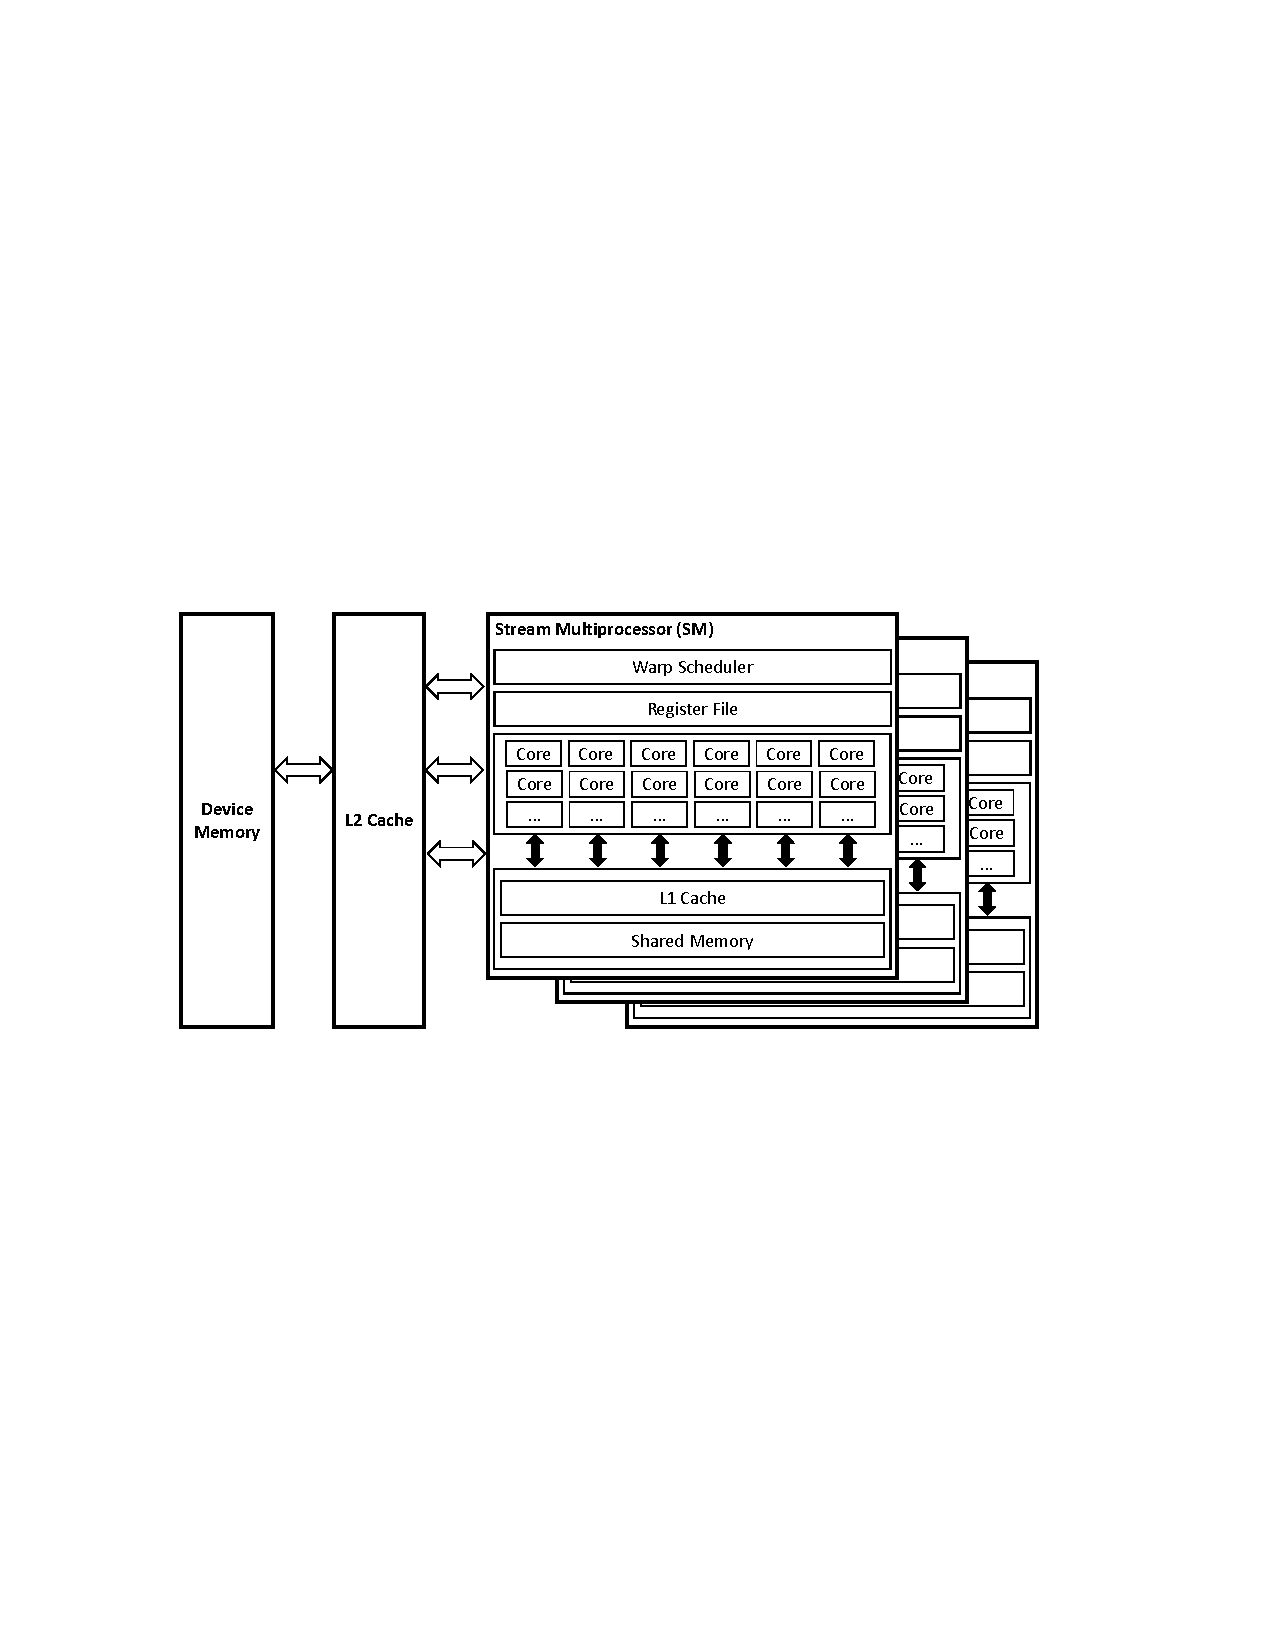
\includegraphics[width=0.5\textwidth]{fig/GPU-arch.pdf}
	\caption{Layout of an NVIDIA GPU architecture}
	\label{fig:arch}
\end{figure}

We focus on introducing the background of NVIDIA GPU architecture in this paper due to its popularity and wide adoption of the CUDA programming language. 
It is noted that our proposed approaches are not unique to NVIDIA GPUs and can be implemented on other GPU architectures as well. Figure~\ref{fig:arch} presents a high-level layout of a NVIDIA GPU. An application written in CUDA executes on GPUs through invoking the \emph{kernel} function. The kernel is organized as a number of \emph{thread blocks}, and one block executes all its threads on a \emph{streaming multiprocessor}, which contains a number of CUDA cores as depicted in the figure. Within a block, threads are divided into \emph{warps} of 32 threads each. 
A CUDA core executes the same instruction of a warp in a lockstep.
Each warp runs independently but can collaborate through different memory types discussed as the following.  

\vspace{1mm}\noindent\textbf{Memory Hierarchy.} Compared CPUs, GPUs are built with large register files to enable massive parallelism. 
For example, NVIDIA GTX 1080 GPUs feature 256KB of register files for each SM. Furthermore, the shared memory, which has similar performance with the L1 cache, can be programmed within a block to facilitate efficient local memory access inside a SM.
The L2 cache is shared among all SMs to speedup memory access to the device memory. The device memory has the largest capacity and the lowest bandwidth in the GPU memory hierarchy.

%GPUs offer an significant better data accessing throughputs than CPUs for two major reasons. 
%First,the device memory has high memory bandwidth, often an order of magnitude faster than RAM.
%Second, GPUs effectively hide memory access latency by warp switching. When a warp is blocked by memory accesses, other warps whose next instruction has its operands ready are eligible to be scheduled for execution. With sufficient threads launched, memory stalls can be minimized or even eliminated \cite{zhang2015mega}.
%Thus, the fast data accessing performance makes GPUs an ideal accelerator for data intensive applications such as hash tables. 

%Data is transferred between CPUs and GPUs (or between two GPU devices) via the PCIe link (Gen 3), which has been the bottleneck of many data-intensive applications \cite{zhang2015mega,kaldewey2012gpu,zhang2013omnidb}. In recent years, there have been many innovations proposed to reduce the overhead of the data transfer, from overlapping PCIe transfer with kernel execution to using hardware acceleration such as PCIe Gen 4 and NVlink \cite{thompto2016power9}. Nonetheless, we omit the discussion on how to minimize this data transfer cost since it is orthogonal to designing an efficient hash table on \emph{one} GPU device.

\vspace{1mm}\noindent\textbf{Optimizing GPU Programs.}
When programming a GPU device, there are several important guidelines to harness GPUs' massive parallelism.
\begin{itemize}
	\item \emph{Minimize Warp Divergence.} Threads in a warp will be serialized if they execute different instructions. To enable maximum parallelism, one needs to minimize branching statements executed within a warp.  
	\item \emph{Coalesced Memory Access.} Warps have a wide cache line size (128 bytes for NVIDIA GPU). The threads are better off to read consecutive memory locations for fully utilizing the device memory bandwidth, otherwise to trigger multiple random accesses for a single read instruction by a warp. 
	\item \emph{Control Resource Usage.} Registers and shared memory are valuable resources to enable fast local memory accesses. Nevertheless, each SM has limited resources (GTX 1080 has 98 KB shared memory and 256KB register files per SM). Overdosing register files or shared memory leads to reduced parallelism on a SM.  
	\item \emph{Atomic Operations.} When facing thread conflicts, an improper locking implementation leads to serious performance degradation. One can leverage the native support of atomic operations \cite{sanders2010cuda} on GPUs to carefully resolve the conflicts and minimize thread spinning.
\end{itemize}